Diante das limitações identificadas, três abordagens foram consideradas para
expandir a capacidade de instrumentação do veículo, comparadas na Tabela~\ref{tab:solucoes-consideradas}.
A literatura sobre sensores sem fio em veículos destaca justamente a redução de
cabeamento, massa e custo de instalação como motivações recorrentes, embora a
confiabilidade do enlace passe a ser uma restrição central de projeto
\cite{tavares2008_wsn_automobiles,rahman2017_intravehicular_wsn,hashemi2014_intracar_multihop_wsn}.

\section{Cabeamento Dedicado}

A primeira opção consiste em aceitar os custos inerentes à arquitetura cabeada e investir na infraestrutura necessária para cada ponto de medição: acopladores rotativos para as rodas, chicotes dedicados para a asa traseira e extensões do chicote principal para outros pontos de difícil acesso. Essa abordagem preserva a arquitetura existente sem exigir nenhum desenvolvimento de \emph{software} ou \emph{hardware} adicional. No entanto, os custos associados a essa solução envolvem restrições financeiras e técnicas.

Do ponto de vista financeiro, a instrumentação de partes móveis rotativas requer acopladores rotativos (\emph{slip rings}) selados para mitigar ruídos elétricos decorrentes da rotação e resistir ao contato com água e poeira. Chicotes voltados ao ambiente veicular de competição costumam exigir conectores circulares selados e condutores com proteções térmicas e químicas adequadas \cite{blatt2020_aquisicao_formula_sae}, os quais possuem custos de aquisição superiores aos de cabos elétricos convencionais. Tecnicamente, embora a conexão física ofereça alta confiabilidade de sinal, o cabeamento físico e suas blindagens térmicas, blindagens eletromagnéticas e suportes mecânicos adicionam peso ao protótipo. Além disso, o direcionamento de fiação ao longo dos braços de suspensão expõe o chicote a esforços dinâmicos constantes. Há também a complexidade de projeto no roteamento tridimensional para evitar pontos de tração nos cabos durante o esterçamento, e a vulnerabilidade à fadiga mecânica dos condutores após ciclos contínuos de movimentação e vibração.

Além desses fatores, o cabeamento dedicado não viabiliza a aquisição de dados no terceiro cenário levantado (sensores externos ao veículo) e impõe limites ao reposicionamento ou expansão futura de sensores.

\section{Sistemas de Aquisição Independentes}

A segunda opção consiste em desenvolver módulos de aquisição autônomos, cada um com sua própria memória local para gravação dos dados. Esses módulos operariam de forma independente do sistema principal, sendo instalados nos pontos de interesse e recuperados após cada sessão de testes para extração dos dados. Para viabilizar a análise conjunta, seria necessário algum mecanismo de sincronização temporal entre os módulos e o sistema embarcado no carro.

Embora essa abordagem elimine a fiação de longa distância até o registrador central, ela desloca a questão de massa e volume físico para os próprios módulos. Cada unidade autônoma requer um invólucro de proteção contra impactos, circuitos de condicionamento de sinal, memória de armazenamento e uma bateria dedicada. A massa combinada desses componentes adiciona peso e volume localizado ao protótipo, o qual pode igualar ou até superar a massa de um chicote elétrico direto de curto comprimento. Adicionalmente, a solução introduz a complexidade de sincronização \emph{offline} (propensa a desvios temporais), a impossibilidade de acompanhar os dados em tempo real durante os testes e o risco de perda total de registros caso ocorra falha de alimentação ou avaria física no módulo.

\section{Solução Sem Fio}

A terceira opção, adotada neste projeto, é o desenvolvimento de uma ponte de comunicação sem fio entre os pontos de medição e o sistema de aquisição existente, conforme esquematizado na Figura~\ref{fig:wcan-semfio}. Nessa abordagem, um nó sensor captura os dados localmente e os transmite por rádio para um nó receptor conectado ao barramento CAN do veículo. O receptor injeta os dados na rede como se fossem provenientes de qualquer outro nó cabeado, tornando a comunicação sem fio transparente para o restante do sistema. Trabalhos de telemetria em Fórmula SAE mostram soluções semelhantes, integrando aquisição de dados e comunicação por rádio com a rede do veículo \cite{zanetti2013_formula_sae_wireless,visconti2019_formula_sae_telemetry,fernandes2022_formula_sae_wifi_can}.

\begin{figure}[htbp]
\centering
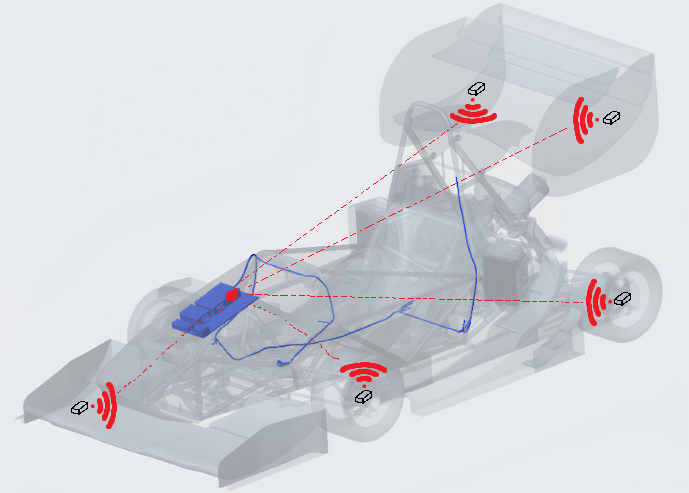
\includegraphics[width=0.85\textwidth]{images/wcan}
\caption{Arquitetura da solução sem fio proposta (WCAN) com transmissão via rádio para receptor central.}
\label{fig:wcan-semfio}
\end{figure}

Essa alternativa elimina a necessidade de roteamento de cabos de comunicação longos e acopladores rotativos, simplificando a instalação em componentes dinâmicos e externos ao carro. Contudo, assim como a aquisição independente, a ponte sem fio introduz peso localizado devido à necessidade de bateria, circuito de condicionamento, rádio e invólucro de proteção em cada nó sensor. Esse conjunto eletrônico pode apresentar massa superior à de uma conexão cabeada local direta de curto comprimento. Além disso, a comunicação sem fio adiciona o gerenciamento de recarga de baterias e o desafio técnico da confiabilidade do enlace, uma vez que a propagação de radiofrequência em ambientes veiculares está sujeita a atenuações e perda de pacotes, apresentando garantias de integridade inferiores às de uma conexão física metálica.

As vantagens e desvantagens de cada uma das alternativas consideradas para expandir a instrumentação estão sintetizadas na Tabela~\ref{tab:solucoes-consideradas}.

\begin{table}[htbp]
\centering
\small
\setlength{\tabcolsep}{4pt}
\renewcommand{\arraystretch}{1.18}
\begin{tabular}{p{0.22\linewidth}|p{0.34\linewidth}|p{0.34\linewidth}}
\hline
Solução & Vantagens & Desvantagens \\
\hline
Cabeamento dedicado &
Preserva a confiabilidade física do barramento CAN e exige baixo esforço de desenvolvimento de \emph{hardware}/\emph{software}. &
Adiciona fiação ao longo da estrutura do veículo; exige acopladores rotativos mecânicos em partes móveis; não atende a sensores externos. \\
\hline
Aquisição independente &
Elimina chicotes elétricos de longa distância; permite instalação em regiões de difícil acesso físico. &
Adiciona massa e volume localizado (bateria, circuitos e gabinete); exige sincronização \emph{offline}; impossibilita visualização em tempo real. \\
\hline
Ponte sem fio &
Remove fiação de longa distância; integra-se diretamente ao CAN existente; permite visualização de dados em tempo real. &
Adiciona massa e volume localizado (bateria, rádio e gabinete); exige desenvolvimento de protocolo de comunicação e tratamento de perda de pacotes. \\
\hline
\end{tabular}
\caption{Comparação das soluções consideradas para expandir a instrumentação do veículo.}
\label{tab:solucoes-consideradas}
\end{table}
